\section*{Výstupní data}

\subsection*{Komprimovaný a zpět dekomprimovaný barevný rastr}
% DCT 2X2
\begin{figure}[H]
    \centering
    \begin{minipage}[b]{0.3\textwidth}
        \centering
        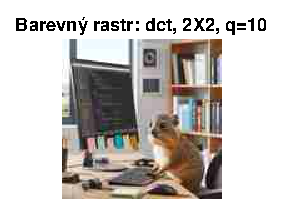
\includegraphics[width=\textwidth]{images/barevny_dct_2X2_q10.eps}
    \end{minipage}
    \hfill
    \begin{minipage}[b]{0.3\textwidth}
        \centering
        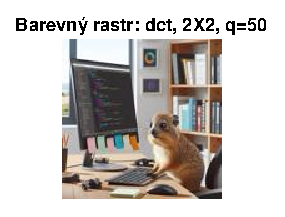
\includegraphics[width=\textwidth]{images/barevny_dct_2X2_q50.eps}
    \end{minipage}
    \hfill
    \begin{minipage}[b]{0.3\textwidth}
        \centering
        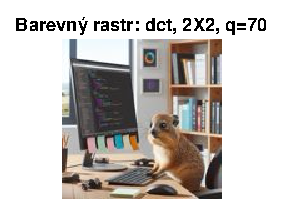
\includegraphics[width=\textwidth]{images/barevny_dct_2X2_q70.eps}
    \end{minipage}
\end{figure}

% DCT NN
\begin{figure}[H]
    \centering
    \begin{minipage}[b]{0.3\textwidth}
        \centering
        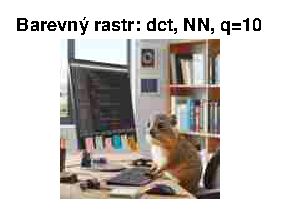
\includegraphics[width=\textwidth]{images/barevny_dct_NN_q10.eps}
    \end{minipage}
    \hfill
    \begin{minipage}[b]{0.3\textwidth}
        \centering
        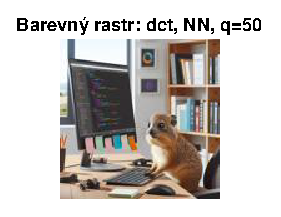
\includegraphics[width=\textwidth]{images/barevny_dct_NN_q50.eps}
    \end{minipage}
    \hfill
    \begin{minipage}[b]{0.3\textwidth}
        \centering
        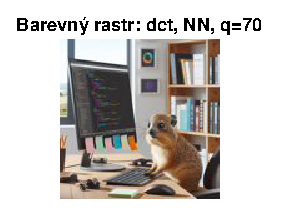
\includegraphics[width=\textwidth]{images/barevny_dct_NN_q70.eps}
    \end{minipage}
\end{figure}

% DWT 2X2
\begin{figure}[H]
    \centering
    \begin{minipage}[b]{0.3\textwidth}
        \centering
        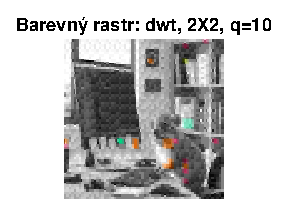
\includegraphics[width=\textwidth]{images/barevny_dwt_2X2_q10.eps}
    \end{minipage}
    \hfill
    \begin{minipage}[b]{0.3\textwidth}
        \centering
        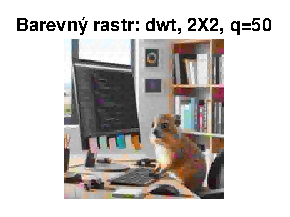
\includegraphics[width=\textwidth]{images/barevny_dwt_2X2_q50.eps}
    \end{minipage}
    \hfill
    \begin{minipage}[b]{0.3\textwidth}
        \centering
        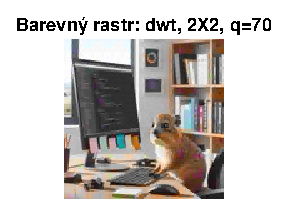
\includegraphics[width=\textwidth]{images/barevny_dwt_2X2_q70.eps}
    \end{minipage}
\end{figure}

% DWT NN
\begin{figure}[H]
    \centering
    \begin{minipage}[b]{0.3\textwidth}
        \centering
        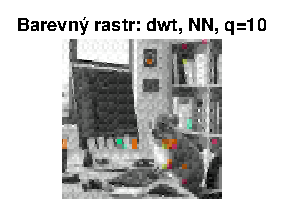
\includegraphics[width=\textwidth]{images/barevny_dwt_NN_q10.eps}
    \end{minipage}
    \hfill
    \begin{minipage}[b]{0.3\textwidth}
        \centering
        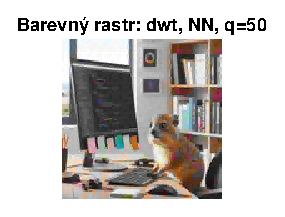
\includegraphics[width=\textwidth]{images/barevny_dwt_NN_q50.eps}
    \end{minipage}
    \hfill
    \begin{minipage}[b]{0.3\textwidth}
        \centering
        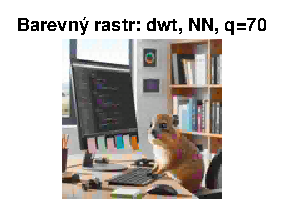
\includegraphics[width=\textwidth]{images/barevny_dwt_NN_q70.eps}
    \end{minipage}
\end{figure}

% FFT 2X2
\begin{figure}[H]
    \centering
    \begin{minipage}[b]{0.3\textwidth}
        \centering
        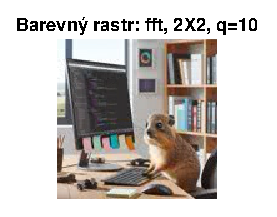
\includegraphics[width=\textwidth]{images/barevny_fft_2X2_q10.eps}
    \end{minipage}
    \hfill
    \begin{minipage}[b]{0.3\textwidth}
        \centering
        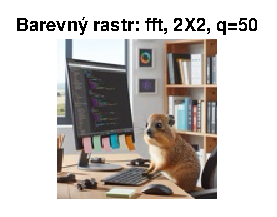
\includegraphics[width=\textwidth]{images/barevny_fft_2X2_q50.eps}
    \end{minipage}
    \hfill
    \begin{minipage}[b]{0.3\textwidth}
        \centering
        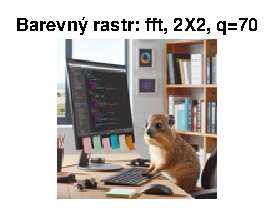
\includegraphics[width=\textwidth]{images/barevny_fft_2X2_q70.eps}
    \end{minipage}
\end{figure}

% FFT NN
\begin{figure}[H]
    \centering
    \begin{minipage}[b]{0.3\textwidth}
        \centering
        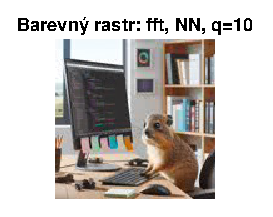
\includegraphics[width=\textwidth]{images/barevny_fft_NN_q10.eps}
    \end{minipage}
    \hfill
    \begin{minipage}[b]{0.3\textwidth}
        \centering
        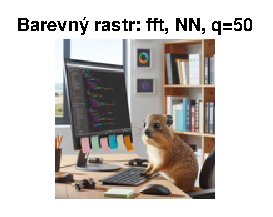
\includegraphics[width=\textwidth]{images/barevny_fft_NN_q50.eps}
    \end{minipage}
    \hfill
    \begin{minipage}[b]{0.3\textwidth}
        \centering
        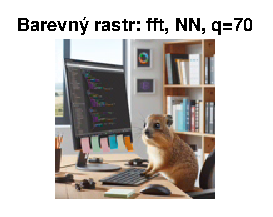
\includegraphics[width=\textwidth]{images/barevny_fft_NN_q70.eps}
    \end{minipage}
\end{figure}

\begin{table}[H]
    \centering
    \textit{Tabulka 1. : Směrodatné odchylky RGB složek pro různé metody transformace, resamplování a kompresní faktory}
    
    \begin{tabular}{|c|c|c|c|c|c|c|c|c|c|c|}
    \hline
    \textbf{Trans.} & \textbf{Res.} & \multicolumn{3}{c|}{\textbf{q = 10}} & \multicolumn{3}{c|}{\textbf{q = 50}} & \multicolumn{3}{c|}{\textbf{q = 70}} \\
    \hline
    & & \(\sigma_R\) & \(\sigma_G\) & \(\sigma_B\) & \(\sigma_R\) & \(\sigma_G\) & \(\sigma_B\) & \(\sigma_R\) & \(\sigma_G\) & \(\sigma_B\) \\
    \hline
    DCT & 2X2 & 14.2314 & 11.5176 & 15.8831 & 8.7282 & 5.6081 & 9.6174 & 7.9765 & 4.8319 & 8.9358 \\ \hline
    DCT & NN  & 14.5588 & 11.5901 & 16.2380 & 9.3283 & 5.8469 & 10.3252 & 8.6363 & 5.0443 & 9.7421 \\ \hline
    DWT & 2X2 & 26.3872 & 21.5015 & 28.8999 & 13.9211 & 9.8437 & 15.9432 & 11.9487 & 8.0544 & 13.5283 \\ \hline
    DWT & NN  & 26.9222 & 21.6850 & 28.8214 & 14.7302 & 9.9927 & 16.6923 & 12.6275 & 8.3376 & 14.3233 \\ \hline
    FFT & 2X2 & 8.9595 & 5.7295 & 9.9961 & 5.7171 & 2.5141 & 6.3373 & 5.5416 & 2.3159 & 6.1004 \\ \hline
    FFT & NN  & 9.6429 & 5.9092 & 10.5269 & 6.9759 & 2.9553 & 7.7958 & 6.7097 & 2.7307 & 7.5133 \\ \hline
    \end{tabular}
\end{table}

%%%%%%%%%%%%%%% šedotónový %%%%%%%%%%%%%%%%%%%%%

\subsection*{Komprimovaný a zpět dekomprimovaný šedotonový rastr}
% DCT 2X2
\begin{figure}[H]
    \centering
    \begin{minipage}[b]{0.3\textwidth}
        \centering
        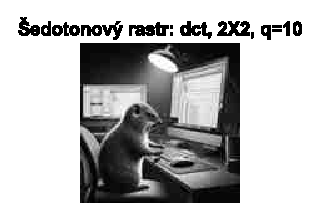
\includegraphics[width=\textwidth]{images/sedo_dct_2X2_q10.eps}
    \end{minipage}
    \hfill
    \begin{minipage}[b]{0.3\textwidth}
        \centering
        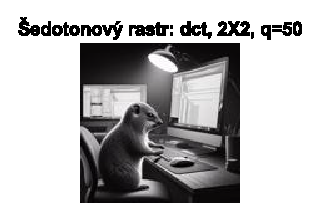
\includegraphics[width=\textwidth]{images/sedo_dct_2X2_q50.eps}
    \end{minipage}
    \hfill
    \begin{minipage}[b]{0.3\textwidth}
        \centering
        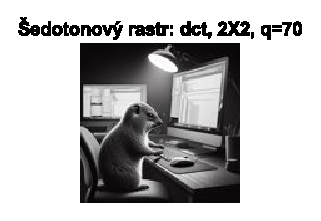
\includegraphics[width=\textwidth]{images/sedo_dct_2X2_q70.eps}
    \end{minipage}
\end{figure}

% DCT NN
\begin{figure}[H]
    \centering
    \begin{minipage}[b]{0.3\textwidth}
        \centering
        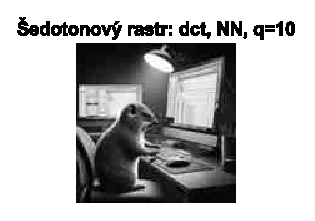
\includegraphics[width=\textwidth]{images/sedo_dct_NN_q10.eps}
    \end{minipage}
    \hfill
    \begin{minipage}[b]{0.3\textwidth}
        \centering
        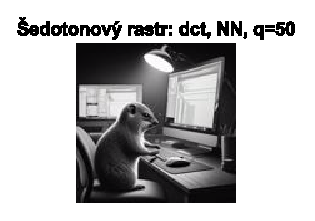
\includegraphics[width=\textwidth]{images/sedo_dct_NN_q50.eps}
    \end{minipage}
    \hfill
    \begin{minipage}[b]{0.3\textwidth}
        \centering
        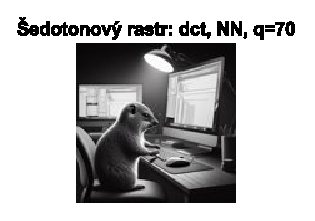
\includegraphics[width=\textwidth]{images/sedo_dct_NN_q70.eps}
    \end{minipage}
\end{figure}

% DWT 2X2
\begin{figure}[H]
    \centering
    \begin{minipage}[b]{0.3\textwidth}
        \centering
        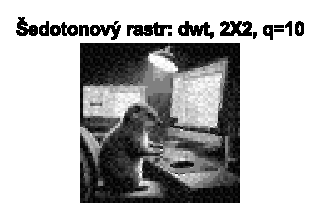
\includegraphics[width=\textwidth]{images/sedo_dwt_2X2_q10.eps}
    \end{minipage}
    \hfill
    \begin{minipage}[b]{0.3\textwidth}
        \centering
        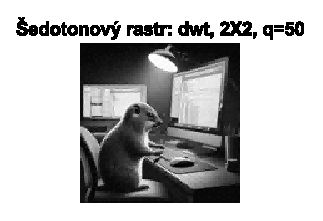
\includegraphics[width=\textwidth]{images/sedo_dwt_2X2_q50.eps}
    \end{minipage}
    \hfill
    \begin{minipage}[b]{0.3\textwidth}
        \centering
        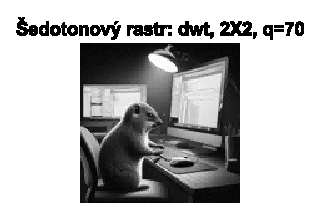
\includegraphics[width=\textwidth]{images/sedo_dwt_2X2_q70.eps}
    \end{minipage}
\end{figure}

% DWT NN
\begin{figure}[H]
    \centering
    \begin{minipage}[b]{0.3\textwidth}
        \centering
        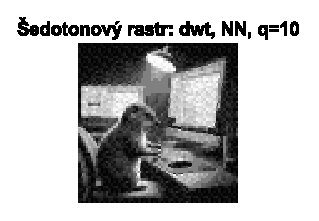
\includegraphics[width=\textwidth]{images/sedo_dwt_NN_q10.eps}
    \end{minipage}
    \hfill
    \begin{minipage}[b]{0.3\textwidth}
        \centering
        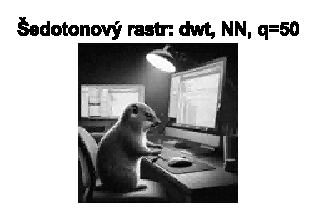
\includegraphics[width=\textwidth]{images/sedo_dwt_NN_q50.eps}
    \end{minipage}
    \hfill
    \begin{minipage}[b]{0.3\textwidth}
        \centering
        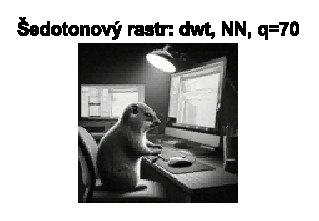
\includegraphics[width=\textwidth]{images/sedo_dwt_NN_q70.eps}
    \end{minipage}
\end{figure}

% FFT 2X2
\begin{figure}[H]
    \centering
    \begin{minipage}[b]{0.3\textwidth}
        \centering
        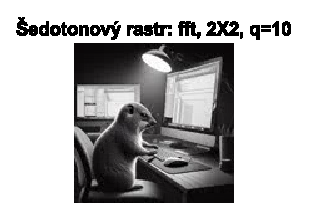
\includegraphics[width=\textwidth]{images/sedo_fft_2X2_q10.eps}
    \end{minipage}
    \hfill
    \begin{minipage}[b]{0.3\textwidth}
        \centering
        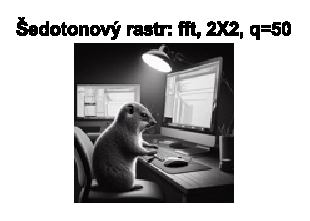
\includegraphics[width=\textwidth]{images/sedo_fft_2X2_q50.eps}
    \end{minipage}
    \hfill
    \begin{minipage}[b]{0.3\textwidth}
        \centering
        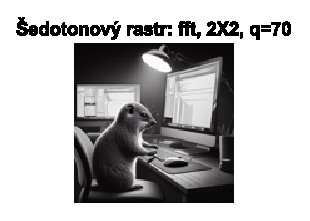
\includegraphics[width=\textwidth]{images/sedo_fft_2X2_q70.eps}
    \end{minipage}
\end{figure}

% FFT NN
\begin{figure}[H]
    \centering
    \begin{minipage}[b]{0.3\textwidth}
        \centering
        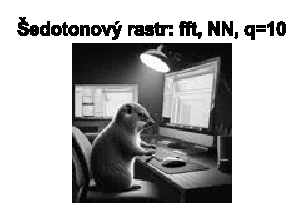
\includegraphics[width=\textwidth]{images/sedo_fft_NN_q10.eps}
    \end{minipage}
    \hfill
    \begin{minipage}[b]{0.3\textwidth}
        \centering
        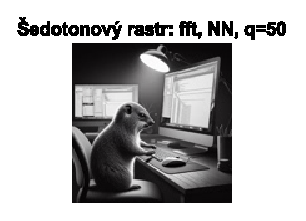
\includegraphics[width=\textwidth]{images/sedo_fft_NN_q50.eps}
    \end{minipage}
    \hfill
    \begin{minipage}[b]{0.3\textwidth}
        \centering
        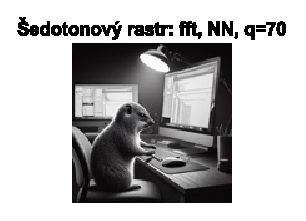
\includegraphics[width=\textwidth]{images/sedo_fft_NN_q70.eps}
    \end{minipage}
\end{figure}

\begin{table}[H]
    \centering
    \textit{Tabulka: Standardní odchylky RGB složek pro různé metody transformace, resamplování a kompresní faktory}
    
    \begin{tabular}{|c|c|c|c|c|c|c|c|c|c|c|}
    \hline
    \textbf{Trans.} & \textbf{Res.} & \multicolumn{3}{c|}{\textbf{q = 10}} & \multicolumn{3}{c|}{\textbf{q = 50}} & \multicolumn{3}{c|}{\textbf{q = 70}} \\
    \hline
    & & \(\sigma_R\) & \(\sigma_G\) & \(\sigma_B\) & \(\sigma_R\) & \(\sigma_G\) & \(\sigma_B\) & \(\sigma_R\) & \(\sigma_G\) & \(\sigma_B\) \\
    \hline
    DCT & 2X2 & 9.9493 & 9.9081 & 9.9058 & 4.7716 & 4.7358 & 4.7866 & 3.8600 & 3.8242 & 3.8465 \\ \hline
    DCT & NN  & 10.0412 & 9.9457 & 9.9770 & 4.7513 & 4.7272 & 4.7839 & 3.8516 & 3.8229 & 3.8393 \\ \hline
    DWT & 2X2 & 19.1238 & 19.0917 & 19.0951 & 8.0933 & 8.0272 & 8.0325 & 6.6940 & 6.6152 & 6.6196 \\ \hline
    DWT & NN  & 19.1797 & 19.1052 & 19.1421 & 8.2075 & 8.0723 & 8.1219 & 6.8302 & 6.6710 & 6.7260 \\ \hline
    FFT & 2X2 & 4.5747 & 4.5585 & 4.5701 & 1.2294 & 1.1626 & 1.2278 & 0.9380 & 0.8555 & 0.9405 \\ \hline
    FFT & NN  & 4.5633 & 4.5571 & 4.5627 & 1.2030 & 1.1579 & 1.1896 & 0.9061 & 0.8477 & 0.8870 \\ \hline
    \end{tabular}
\end{table}